%%%%%%%%%%%%%%%%%%%%%%%%%%%%%%%%%%%%%%%%%%%%%%%%%%%%%%%%%%%%%%%%%%%%%%%%%%%%%%%%
% Set Night Light
%%%%%%%%%%%%%%%%%%%%%%%%%%%%%%%%%%%%%%%%%%%%%%%%%%%%%%%%%%%%%%%%%%%%%%%%%%%%%%%%
\chapter{Set Night Light} \label{Set Night Light}
\vspace{-10ex}\mSN{syml}\vskip 8ex

%%%%%%%%%%%%%%%%%%%%%%%%%%%%%%%%%%%%%%%%%%%%%%%%%%%%%%%%%%%%%%%%%%%%%%%%%%%%%%%%
% Introduction
%%%%%%%%%%%%%%%%%%%%%%%%%%%%%%%%%%%%%%%%%%%%%%%%%%%%%%%%%%%%%%%%%%%%%%%%%%%%%%%%
\section{Introduction}

Allows for setting any of the \num{3} configurable night light colors using
any of \num{3} methods.

\par\medskip

The \cLi{f} is composed of \num{16}
\href{https://en.wikipedia.org/wiki/RGB\_color\_model}{RGB} LEDs.  Each LED is
composed of a Red, a Green and a Blue pixel.  The color of each LED is
determined by the blend of these pixels.

\par\medskip

There are a number of preset colors that can be chosen from.  Additionally,
the color can be customized by either selecting the individual values for the
Red, Green and Blue pixels or by selecting
\href{https://en.wikipedia.org/wiki/HSL\_and\_HSV}{HSB} values -
Hue, Saturation and Brightness.

\par\medskip

It is the \mTe{f} mode when the \cRs{f} is in the \dRi{f} position.

\par\medskip

There are a few ways to get to \mSN{f} depending on which direction the
\cRs{f} is pointing and which mode the device is currently in.  The most
straightforward way is:

\begin{enumerate}
  \item \aTu{f} the \cRs{f} to the \dRi{f}.
  \item \aPH{f} the \cEs{f} until \symD{>>>>} is blinking on the
    \cDi{f} then \aRe{f}.
\end{enumerate}

\begin{table}[H]
\ers{3}
\centering
\begin{tabu} { X[1,c,m] | X[2,c,m] | X[1,c,m] }
  \thrule
  \thbi{Position} & \thbi{Mode} & \thbi{Action} \\ \mrule

  \sMi & \multirow{2}{*}[-1mm]{\mode{s}{ANY}}
    & $\hskip 3mm$ \sMtoR \\ \dcrule{1}{1} \dcrule{3}{3}
  \sLe & & \sLtoR \\ \mdrule

  \multirow{2}{*}[-2mm]{\sRi} & \mTi{sym}
    & \multirow{2}{*}[-2mm]{\sTer} \\ \dcrule{2}{2}
  & \mPS{sym} & \\

  \bhrule
\end{tabu}
\caption{Set Night Light - Mode}
\end{table}

\pagebreak

A few items of note:

\begin{itemize}
  \item The night light number initially loaded will be the one currently
    displayed if the night light in on.
  \item When using a different method from the one used previously
    to set the color, an attempt will be made to get the settings as
    close to the color as possible.
  \item The color will be updated in real time and shown in the \cLi{f} window.
  \item When using either RGB or HSB, you will \hyperref[Double-Click]{\aDC{f}}
    the \cEs{f} to finish.  It's done this way because it is assumed that one
    will likely want to go through the process a number of times to fine tune
    the color.
  \item To \aReset{f} and start over from the top menu, \aPH{f} the \cEs{f}
    until you see \symD{<<<<} blink on the \cDi{f}.
\end{itemize}

%%%%%%%%%%%%%%%%%%%%%%%%%%%%%%%%%%%%%%%%%%%%%%%%%%%%%%%%%%%%%%%%%%%%%%%%%%%%%%%%
% Overview
%%%%%%%%%%%%%%%%%%%%%%%%%%%%%%%%%%%%%%%%%%%%%%%%%%%%%%%%%%%%%%%%%%%%%%%%%%%%%%%%
\section{Overview}

There are a number of states \mSN{f} can be in and are explained in the next
sections.

\begin{table}[H]
\ers{2}
\centering
\begin{tabu}{ X[1,c,m] | X[3,l,m] }
  \thrule
  \thbi{State} & \thbi{Description} \\ \mrule

  \sSNMN{sym} & Select one of the three night light colors
    you want to set. \\ \drule{2}
  \sSNMC{sym} & Select the method for setting the color. \\ \drule{2}
  \sSNCI{sym} & Set the color by selecting one of many
    preset colors. \\ \drule{2}
  \sSNRe{sym} & Set the Red pixel value. \\ \drule{2}
  \sSNGr{sym} & Set the Green pixel value. \\ \drule{2}
  \sSNBl{sym} & Set the Blue pixel value. \\ \drule{2}
  \sSNHu{sym} & Set a Hue value. \\ \drule{2}
  \sSNSa{sym} & Set a Saturation value. \\ \drule{2}
  \sSNBr{sym} & Set a Brightness value. \\ \drule{2}
  \sSNDo{sym} & Display settings values. \\
  \bhrule
\end{tabu}
\caption{Set Night Light - States}
\end{table}

To progress through the states, you will first \aTu{f} the \cEs{f} to select
one of the \num{3} configurable night light colors, \mSNOn{f}, \mSNTw{f} or
\mSNTh{f}, then \aPR{f} the \cEs{f}.

\ase{1}{{ c c c c c }}{%
& & \eSel{sym}{} \mSNOn{sym} & & \\ \dcrule{3}{3}
\sSNMN{sym} & \sTu & \eSel{sym}{} \mSNTw{sym} & \sPR & \sSNMC{sym} \\ \dcrule{3}{3}
& & \eSel{sym}{} \mSNTh{sym} & & \\}

The \sSNMC{f} has three options for setting the color.

\begin{table}[H]
\ers{0.1}
\centering
\begin{tabu} { c c }
  \thi{Option} & \thi{Display} \\ \mrule
  \mSNCo{sym} & \symD{CoLr} \\
  \mSNRGB{sym} & \symD{rgb!} \\
  \mSNHSB{sym} & \symD{HSb!} \\
\end{tabu}
\end{table}

\aTu{f} the \cEs{f} to select the method for setting the color of the chosen
night light then \aPR{f}.

\ase{1}{{ c c c c c }}{%
& & \eSel{sym}{} \mSNCo{sym} & & \sSNCI{sym} \\ \dcrule{3}{3} \dcrule{5}{5}
\sSNMC{sym} & \sTu & \eSel{sym}{} \mSNRGB{sym}
  & \sPR & \sSNRe{sym} \\ \dcrule{3}{3} \dcrule{5}{5}
& & \eSel{sym}{} \mSNHSB{sym} & & \sSNHu{sym} \\}

%%%%%%%%%%%%%%%%%%%%%%%%%%%%%%%%%%%%%%%%%%%%%%%%%%%%%%%%%%%%%%%%%%%%%%%%%%%%%%%%
% Overview - Preset
%%%%%%%%%%%%%%%%%%%%%%%%%%%%%%%%%%%%%%%%%%%%%%%%%%%%%%%%%%%%%%%%%%%%%%%%%%%%%%%%
\mSNCo{sym} \par\medskip

Select a preset color.

\par\medskip

This menu option is probably the easiest to use for setting the color.  There
are over \num{100} colors to choose from.  There is one state - \sSNCI{f} - when
taking this path before finishing.

\as{{ c c c c }}{ \sSNCI{sym} & \sTu & \sPR & \sSNDo{sym} \\}

%%%%%%%%%%%%%%%%%%%%%%%%%%%%%%%%%%%%%%%%%%%%%%%%%%%%%%%%%%%%%%%%%%%%%%%%%%%%%%%%
% Overview - RGB
%%%%%%%%%%%%%%%%%%%%%%%%%%%%%%%%%%%%%%%%%%%%%%%%%%%%%%%%%%%%%%%%%%%%%%%%%%%%%%%%
\mSNRGB{sym} \par\medskip

Create a color by selecting individual \sSNRe{f}, \sSNGr{f} and \sSNBl{f} pixel
values.

\par\medskip

This method allows you to select values for the individual \sSNRe{f}, \sSNGr{f}
and \sSNBl{f} pixels of the LEDs.

\ase{1}{{ c c c c c c c c c c }}{%
  \multirow{2}{*}{\sSNRe{sym}}
  & \multirow{2}{*}{\sTu}
  & \multirow{2}{*}{\sPR}
  & \multirow{2}{*}{\sSNGr{sym}}
  & \multirow{2}{*}{\sTu}
  & \multirow{2}{*}{\sPR}
  & \multirow{2}{*}{\sSNBl{sym}}
  & \multirow{2}{*}{\sTu} & \sPR & \sSNRe{sym} \\ \dcrule{9}{10}
& & & & & & & & \sDC & \sSNDo{sym} \\}

\pagebreak
At any time you can \aDC{f} to finish.

\ase{1}{{ c c c c c c c c c c }}{%
& & \sDC & \sSNDo{sym} \\ \dcrule{3}{7}
\sSNRe{sym} & \sTu
  & \multirow{2}{*}{\sPR}
  & \multirow{2}{*}{\sSNGr{sym}}
  & \multirow{2}{*}{\sTu} & \sDC & \sSNDo{sym} \\ \dcrule{6}{10}
& & & & & \sPR & \sSNBl{sym} & \sTu & \sDC & \sSNDo{sym} \\}

%%%%%%%%%%%%%%%%%%%%%%%%%%%%%%%%%%%%%%%%%%%%%%%%%%%%%%%%%%%%%%%%%%%%%%%%%%%%%%%%
% Overview - HSB
%%%%%%%%%%%%%%%%%%%%%%%%%%%%%%%%%%%%%%%%%%%%%%%%%%%%%%%%%%%%%%%%%%%%%%%%%%%%%%%%
\mSNHSB{sym} \par\medskip

Create a color by selecting \sSNHu{f}, \sSNSa{f} and \sSNBr{f} values.

\par\medskip

This method allows you to set the night light color by individually selecting
\sSNHu{f}, \sSNSa{f} and \sSNBr{f} values.

\ase{1}{{ c c c c c c c c c c }}{%
  \multirow{2}{*}{\sSNHu{sym}}
  & \multirow{2}{*}{\sTu}
  & \multirow{2}{*}{\sPR}
  & \multirow{2}{*}{\sSNSa{sym}}
  & \multirow{2}{*}{\sTu}
  & \multirow{2}{*}{\sPR}
  & \multirow{2}{*}{\sSNBr{sym}}
  & \multirow{2}{*}{\sTu} & \sPR & \sSNHu{sym} \\ \dcrule{9}{10}
& & & & & & & & \sDC & \sSNDo{sym} \\}

At any time you can \aDC{f} to finish.

\ase{1}{{ c c c c c c c c c c }}{%
& & \sDC & \sSNDo{sym} \\ \dcrule{3}{7}
\sSNHu{sym} & \sTu
  & \multirow{2}{*}{\sPR}
  & \multirow{2}{*}{\sSNSa{sym}}
  & \multirow{2}{*}{\sTu} & \sDC & \sSNDo{sym} \\ \dcrule{6}{10}
& & & & & \sPR & \sSNBr{sym} & \sTu & \sDC & \sSNDo{sym} \\}

%%%%%%%%%%%%%%%%%%%%%%%%%%%%%%%%%%%%%%%%%%%%%%%%%%%%%%%%%%%%%%%%%%%%%%%%%%%%%%%%
% Color Menu
%%%%%%%%%%%%%%%%%%%%%%%%%%%%%%%%%%%%%%%%%%%%%%%%%%%%%%%%%%%%%%%%%%%%%%%%%%%%%%%%
\section{Color Menu} \sSNMN{syml}

Select one of the three night light colors you want to configure.

\par\medskip

To select one of the night light colors, \aTu{f} the \cEs{f} then \aPR{f}
to go on to select a method for setting the color of the night light selected.
As you cycle through the numbers, the current color of that number will light up
the \cLi{f} window.

%\ase{1}{{ c c c c c c }}{%
%& & \eLi{sym}{} \mSNOn{sym}
%  & & \eSel{sym}{} \mSNOn{sym} & \\ \dcrule{3}{3} \dcrule{5}{5}
%\sSNMN{sym} & \sTu & \eLi{sym}{} \mSNTw{sym}
%  & \sPR & \eSel{sym}{} \mSNTw{sym} & \sSNMC{sym} \\ \dcrule{3}{3} \dcrule{5}{5}
%& & \eLi{sym}{} \mSNTh{sym} & & \eSel{sym}{} \mSNTh{sym} & \\}

\as{{c c c c}}{%
  \multirow{2}{*}{\sSNMN{sym}} & \sTu & \sPR & \multirow{2}{*}{\sSNMC{sym}} \\
  & \eUp{sym}{COLOR} & \eSel{sym}{COLOR} & \\}

%%%%%%%%%%%%%%%%%%%%%%%%%%%%%%%%%%%%%%%%%%%%%%%%%%%%%%%%%%%%%%%%%%%%%%%%%%%%%%%%
% Method Menu
%%%%%%%%%%%%%%%%%%%%%%%%%%%%%%%%%%%%%%%%%%%%%%%%%%%%%%%%%%%%%%%%%%%%%%%%%%%%%%%%
\pagebreak
\section{Method Menu} \sSNMC{syml}

Select a method for setting a night light's color.

\par\medskip

There are \num{3} ways to set the color of the selected night light.

\begin{table}[H]
\ers{3}
\centering
\begin{tabu} { X[1,c,m] | X[1,c,m] | X[3,l,m] }
  \thrule
  \thbi{Method} & \thbi{Display} & \thbi{Description} \\ \mrule
  \mSNCo{sym} & \sDl{CoLr} & Select a \sSNCI{f} from a number of preset colors. \\ \drule{3}
  \mSNRGB{sym} & \sDl{rgb!} & Create a color by selecting the
    individual \sSNRe{f}, \sSNGr{f} and \sSNBl{f} pixel values. \\ \drule{3}
  \mSNHSB{sym} & \sDl{HSb!} & Create a color by selecting
    \sSNHu{f}, \sSNSa{f} and \sSNBr{f} values. \\
  \bhrule
\end{tabu}
\end{table}

To select a method, \aTu{f} the \cEs{f} to choose one of the above, then \aPR{f}
to select the method and move on to the first state of the chosen method.

\as{{m{3.5in} m{2in}}}{%
\begin{tabu}{c c c}
  \multirow{2}{*}{\sSNMC{sym}} & \sTu & \sPR \\
  & \eUp{sym}{METHOD} & \eSel{sym}{METHOD}
\end{tabu} &
\begin{tabu}{c c c}
  \mSNCo{sym} & $\longrightarrow$ & \sSNCI{sym} \\ \drule{3}
  \mSNRGB{sym} & $\longrightarrow$ & \sSNRe{sym} \\ \drule{3}
  \mSNHSB{sym} & $\longrightarrow$ & \sSNHu{sym}
\end{tabu} \\}

%%%%%%%%%%%%%%%%%%%%%%%%%%%%%%%%%%%%%%%%%%%%%%%%%%%%%%%%%%%%%%%%%%%%%%%%%%%%%%%%
% Color
%%%%%%%%%%%%%%%%%%%%%%%%%%%%%%%%%%%%%%%%%%%%%%%%%%%%%%%%%%%%%%%%%%%%%%%%%%%%%%%%
\section{Color} \sSNCI{syml}

Select a color from a number of preset colors.

\par\medskip

There over \num{100} preset colors to choose from.  The ordering may seem
somewhat random but you'll notice that many colors types are grouped
together.  As you \aTu{f} the \cEs{f}, the current color will light up 
in the \cLi{f} window and its index\slash number will be shown on the \cDi{f}.
There is no correlation between the index and the color other than its
position in the list of preset colors.

\par\medskip

The first and last colors are \textit{white} and \textit{black} respectively.
To quickly get to the last color from the first, turn \textit{counter-clockwise}
and \num{1} will wrap to the last number.

\par\medskip

To select a color, \aTu{f} the \cEs{f} to cycle through the colors then
\aPR{f} to select a color and finish.

\as{{c c c c c}}{%
\multirow{2}{*}{\sSNCI{sym}}
  & \sTu & \multirow{2}{*}{\sPR} & \eSe{sym}{COLOR}
  & \multirow{2}{*}{\sSNDo{sym}} \\
& \eUp{sym}{} & & \eSa{sym}{COLOR} & \\}

%%%%%%%%%%%%%%%%%%%%%%%%%%%%%%%%%%%%%%%%%%%%%%%%%%%%%%%%%%%%%%%%%%%%%%%%%%%%%%%%
% RGB
%%%%%%%%%%%%%%%%%%%%%%%%%%%%%%%%%%%%%%%%%%%%%%%%%%%%%%%%%%%%%%%%%%%%%%%%%%%%%%%%
\section{RGB} \mSNRGB{syml}

This method allows you to select values for the individual \sSNRe{f}, \sSNGr{f}
and \sSNBl{f} pixels of the LEDs.\footnote{ More detailed information on the RGB
color model can be found
\href{https://en.wikipedia.org/wiki/RGB\_color\_model}{here}.}

\par\medskip

The allowable values for each range from \num{0} to \num{255}, but note that
the values are displayed in hexadecimal.\footnote{ See
\hyperref[Hexadecimal]{Hexadecimal} in the Appendix.} Hexadecimal value
\mono{FF} is equivalent to the decimal value \num{255}. All you really need to
know is that turning \textit{counter-clockwise} will \textit{decrease} the
intensity of the RGB pixel being set and turning \textit{clockwise} will
\textit{increase} the intensity.

\par\medskip

A few items of note:

\begin{itemize}
  \item Setting \sSNRe{f}, \sSNGr{f} and \sSNBl{f} to \mono{FF} will give you
    \textit{white}.
  \item Setting \sSNRe{f}, \sSNGr{f} and \sSNBl{f} to \mono{00} will give you
    \textit{black}.  This can be utilized in \mCl{f} mode so you can \aTu{f}
    the \cEs{f} instead of having to \aPR{f} the \cEs{f} to turn the night
    light off.
  \item As you change an \mSNRGB{f} value, the color will be updated in the
    \cLi{f} area.
  \item To finish, you will \aDC{f} the \cEs{f}.  This can be done in any of the
    \mSNRGB{f} states.
\end{itemize}

Unlike other settings, a single \aPR{f} of the \cEs{f} will continue to cycle
through the \sSNRe{f}, \sSNGr{f} and \sSNBl{f} states to give you an opportunity
to go through the process again and tune the values to get the color you want.  A
\aDC{f} of the \cEs{f} will get you out of this loop and finish.

\par\medskip

\info{Depending on the color set, there may be some desyncing between the
\cDi{f} and \cLi{f} at low brightness levels.  This is because given different
values for the pixels, they may drop out before the \cDi{f} turns off and
may be slightly delayed after the \cDi{f} turns on when turning the \cBr{f}.}

\info{Depending on the color set, you may notice that at low brightness levels
the color changes.  This is because at some point one of the RGB pixels drops
out or turns off before the others.}

%%%%%%%%%%%%%%%%%%%%%%%%%%%%%%%%%%%%%%%%%%%%%%%%%%%%%%%%%%%%%%%%%%%%%%%%%%%%%%%%
% RGB - Red
%%%%%%%%%%%%%%%%%%%%%%%%%%%%%%%%%%%%%%%%%%%%%%%%%%%%%%%%%%%%%%%%%%%%%%%%%%%%%%%%
\subsection{Red} \sSNRe{syml}

Select the intensity of the \sSNRe{f} pixel.

\par\medskip

The \cDi{f} will show the following

\begin{figure}[H]
\centering
  \sDl{r!:FF}
\end{figure}

and the number on the \textit{right} side of the \textit{colon} will be
\textit{blinking}.  To select the \sSNRe{f} value, \aTu{f} the \cEs{f} then
either:

\begin{enumerate}
  \item \aPR{f} the \cEs{f} to cache the value and move on to \sSNGr{f},
    \textit{or}
  \item \aDC{f} the \cEs{f} to set, save and finish.
\end{enumerate}

\as{{m{1.25in} m{2.1in}}}{%
\begin{tabu}{c c}
  \multirow{2}{*}{\sSNRe{sym}} & \sTu \\
  & \eUp{sym}{}
\end{tabu} &
\begin{tabu}{c c c}
  \sPR & \eCa{sym}{RED} & \sSNGr{sym} \\ \drule{3}
  \multirow{2}{*}{\sDC} & \eSe{sym}{COLOR} & \multirow{2}{*}{\sSNDo{sym}} \\
  & \eSa{sym}{COLOR} &
\end{tabu} \\}

%%%%%%%%%%%%%%%%%%%%%%%%%%%%%%%%%%%%%%%%%%%%%%%%%%%%%%%%%%%%%%%%%%%%%%%%%%%%%%%%
% RGB - Green
%%%%%%%%%%%%%%%%%%%%%%%%%%%%%%%%%%%%%%%%%%%%%%%%%%%%%%%%%%%%%%%%%%%%%%%%%%%%%%%%
\subsection{Green} \sSNGr{syml}

Select the intensity of the \sSNGr{f} pixel.

\par\medskip

The \cDi{f} will show the following

\begin{figure}[H]
\centering
  \sDl{g!:FF}
\end{figure}

and the number on the \textit{right} side of the \textit{colon} will be
\textit{blinking}.  To select the \sSNGr{f} value, \aTu{f} the \cEs{f} then
either:

\begin{enumerate}
  \item \aPR{f} the \cEs{f} to cache the value and move on to \sSNBl{f},
    \textit{or}
  \item \aDC{f} the \cEs{f} to set, save and finish.
\end{enumerate}

\as{{m{1.25in} m{2.1in}}}{%
\begin{tabu}{c c}
  \multirow{2}{*}{\sSNGr{sym}} & \sTu \\
  & \eUp{sym}{}
\end{tabu} &
\begin{tabu}{c c c}
  \sPR & \eCa{sym}{GREEN} & \sSNBl{sym} \\ \drule{3}
  \multirow{2}{*}{\sDC} & \eSe{sym}{COLOR} & \multirow{2}{*}{\sSNDo{sym}} \\
  & \eSa{sym}{COLOR} &
\end{tabu} \\}

%%%%%%%%%%%%%%%%%%%%%%%%%%%%%%%%%%%%%%%%%%%%%%%%%%%%%%%%%%%%%%%%%%%%%%%%%%%%%%%%
% RGB - Blue
%%%%%%%%%%%%%%%%%%%%%%%%%%%%%%%%%%%%%%%%%%%%%%%%%%%%%%%%%%%%%%%%%%%%%%%%%%%%%%%%
\subsection{Blue} \sSNBl{syml}

Select the intensity of the \sSNBl{f} pixel.

\par\medskip

The \cDi{f} will show the following

\begin{figure}[H]
\centering
  \sDl{b!:FF}
\end{figure}

and the number on the \textit{right} side of the \textit{colon} will be
\textit{blinking}.  To select the \sSNBl{f} value, \aTu{f} the \cEs{f} then
either:

\begin{enumerate}
  \item \aPR{f} the \cEs{f} to cache the value and cycle back to \sSNRe{f},
    \textit{or}
  \item \aDC{f} the \cEs{f} to set, save and finish.
\end{enumerate}

\as{{m{1.25in} m{2.1in}}}{%
\begin{tabu}{c c}
  \multirow{2}{*}{\sSNBl{sym}} & \sTu \\
  & \eUp{sym}{}
\end{tabu} &
\begin{tabu}{c c c}
  \sPR & \eCa{sym}{BLUE} & \sSNRe{sym} \\ \drule{3}
  \multirow{2}{*}{\sDC} & \eSe{sym}{COLOR} & \multirow{2}{*}{\sSNDo{sym}} \\
  & \eSa{sym}{COLOR} &
\end{tabu} \\}

%%%%%%%%%%%%%%%%%%%%%%%%%%%%%%%%%%%%%%%%%%%%%%%%%%%%%%%%%%%%%%%%%%%%%%%%%%%%%%%%
% HSB
%%%%%%%%%%%%%%%%%%%%%%%%%%%%%%%%%%%%%%%%%%%%%%%%%%%%%%%%%%%%%%%%%%%%%%%%%%%%%%%%
\section{HSB} \mSNHSB{syml}

This method allows you to set the night light color by individually selecting
\sSNHu{f}, \sSNSa{f} and \sSNBr{f} values.\footnote{ More detailed
information on the HSB color space can be found
\href{https://en.wikipedia.org/wiki/HSL\_and\_HSV}{here}.}

\par\medskip

The allowable values for each range from \num{0} to \num{255}, but note that the
values are displayed in hexadecimal.\footnote{ See
\hyperref[Hexadecimal]{Hexadecimal} in the Appendix.} Hexadecimal value
\mono{FF} is equivalent to the decimal value \num{255}. All you really need to
know is that turning \textit{counter-clockwise} will \textit{decrease} the
HSB value being set and turning \textit{clockwise} will \textit{increase} it.

\par\medskip

A few items of note:

\begin{itemize}
  \item Changing the \sSNHu{f} essentially changes the color which may make
    using this method easier than the \mSNRGB{f} method.
  \item Lowering the \sSNSa{f} value will \textit{whiten} the \sSNHu{f}.
  \item Try not to change the \sSNBr{f} from \mono{FF} since the
    brightness of the \cLi{f} is adjustable via the \cBr{f}.
  \item As you change an \mSNHSB{f} value, the color will be updated in the
    \cLi{f} area.
  \item To finish, you will \aDC{f} the \cEs{f}.  This can be done
    in any of the \mSNHSB{f} states.
\end{itemize}

Like \mSNRGB{f}, a single \aPR{f} of the \cEs{f} will continue to cycle through
the \sSNHu{f}, \sSNSa{f} and \sSNBr{f} states to give you an opportunity to go
through the process again and tune the values to get the color you want.  A
\aDC{f} of the \cEs{f} will get you out of this loop and finish.

\par\medskip

\info{Depending on the color set, there may be some desyncing between the
\cDi{f} and \cLi{f} at low brightness levels.  This is because given different
values for the pixels, they may drop out before the \cDi{f} turns off and
may be slightly delayed after the \cDi{f} turns on when turning the \cBr{f}.}

\info{Depending on the values set, you may notice that at low brightness levels
the color changes.  This is because at some point one of the RGB pixels drops
out or turns off before the others.}

%%%%%%%%%%%%%%%%%%%%%%%%%%%%%%%%%%%%%%%%%%%%%%%%%%%%%%%%%%%%%%%%%%%%%%%%%%%%%%%%
% HSB - Hue
%%%%%%%%%%%%%%%%%%%%%%%%%%%%%%%%%%%%%%%%%%%%%%%%%%%%%%%%%%%%%%%%%%%%%%%%%%%%%%%%
\subsection{Hue} \sSNHu{syml}

Select a \sSNHu{f} value.

\par\medskip

The \cDi{f} will show the following

\begin{figure}[H]
\centering
  \sDl{H!:00}
\end{figure}

and the number on the \textit{right} side of the \textit{colon} will be
\textit{blinking}.  To select the \sSNHu{f} value, \aTu{f} the \cEs{f} then
either:

\begin{enumerate}
  \item \aPR{f} the \cEs{f} to cache the value and move on to \sSNSa{f},
    \textit{or}
  \item \aDC{f} the \cEs{f} to set, save and finish.
\end{enumerate}

\as{{m{1.25in} m{2.4in}}}{%
\begin{tabu}{c c}
  \multirow{2}{*}{\sSNHu{sym}} & \sTu \\
  & \eUp{sym}{}
\end{tabu} &
\begin{tabu}{c c c}
  \sPR & \eCa{sym}{HUE} & \sSNSa{sym} \\ \drule{3}
  \multirow{2}{*}{\sDC} & \eSe{sym}{COLOR} & \multirow{2}{*}{\sSNDo{sym}} \\
  & \eSa{sym}{COLOR} &
\end{tabu} \\}

%%%%%%%%%%%%%%%%%%%%%%%%%%%%%%%%%%%%%%%%%%%%%%%%%%%%%%%%%%%%%%%%%%%%%%%%%%%%%%%%
% HSB - Saturateion
%%%%%%%%%%%%%%%%%%%%%%%%%%%%%%%%%%%%%%%%%%%%%%%%%%%%%%%%%%%%%%%%%%%%%%%%%%%%%%%%
\pagebreak
\subsection{Saturation} \sSNSa{syml}

Select a \sSNSa{f} value.

\par\medskip

The \cDi{f} will show the following

\begin{figure}[H]
\centering
  \sDl{S!:00}
\end{figure}

and the number on the \textit{right} side of the \textit{colon} will be
\textit{blinking}.  To select the \sSNSa{f} value, \aTu{f} the \cEs{f} then
either:

\begin{enumerate}
  \item \aPR{f} the \cEs{f} to cache the value and move on to \sSNBr{f},
    \textit{or}
  \item \aDC{f} the \cEs{f} to set, save and finish.
\end{enumerate}

\as{{m{1.7in} m{2.75in}}}{%
\begin{tabu}{c c}
  \multirow{2}{*}{\sSNSa{sym}} & \sTu \\
  & \eUp{sym}{}
\end{tabu} &
\begin{tabu}{c c c}
  \sPR & \eCa{sym}{SATURATION} & \sSNBr{sym} \\ \drule{3}
  \multirow{2}{*}{\sDC} & \eSe{sym}{COLOR} & \multirow{2}{*}{\sSNDo{sym}} \\
  & \eSa{sym}{COLOR} &
\end{tabu} \\}

%%%%%%%%%%%%%%%%%%%%%%%%%%%%%%%%%%%%%%%%%%%%%%%%%%%%%%%%%%%%%%%%%%%%%%%%%%%%%%%%
% HSB - Brightness
%%%%%%%%%%%%%%%%%%%%%%%%%%%%%%%%%%%%%%%%%%%%%%%%%%%%%%%%%%%%%%%%%%%%%%%%%%%%%%%%
\subsection{Brightness} \sSNBr{syml}

Select a \sSNBr{f} value.

\par\medskip

The \cDi{f} will show the following

\begin{figure}[H]
\centering
  \sDl{b!:00}
\end{figure}

and the number on the \textit{right} side of the \textit{colon} will be
\textit{blinking}.  To select the \sSNBr{f} value, \aTu{f} the \cEs{f} then
either:

\begin{enumerate}
  \item \aPR{f} the \cEs{f} to cache the value and cycle back to \sSNHu{f},
    \textit{or}
  \item \aDC{f} the \cEs{f} to set, save and finish.
\end{enumerate}

\as{{m{1.7in} m{2.45in}}}{%
\begin{tabu}{c c}
  \multirow{2}{*}{\sSNBr{sym}} & \sTu \\
  & \eUp{sym}{}
\end{tabu} &
\begin{tabu}{c c c}
  \sPR & \eCa{sym}{BRIGHTNESS} & \sSNHu{sym} \\ \drule{3}
  \multirow{2}{*}{\sDC} & \eSe{sym}{COLOR} & \multirow{2}{*}{\sSNDo{sym}} \\
  & \eSa{sym}{COLOR} &
\end{tabu} \\}

%%%%%%%%%%%%%%%%%%%%%%%%%%%%%%%%%%%%%%%%%%%%%%%%%%%%%%%%%%%%%%%%%%%%%%%%%%%%%%%%
% Done
%%%%%%%%%%%%%%%%%%%%%%%%%%%%%%%%%%%%%%%%%%%%%%%%%%%%%%%%%%%%%%%%%%%%%%%%%%%%%%%%
\section{Done} \sSNDo{syml}

This state allows for review of the settings which are shown on the \cDi{f}.

\par\medskip

At this point you can start over or go to some other mode.  To start over and go
back to the \sSNMN{f}, \aPR{f} the \cEs{f}.

\as{{c c c}}{\sSNDo{sym} & \sPR & \sSNMN{sym} \\}

To go to, say \mCl{f} mode, \aTu{f} the \cRs{f} to the \dMi{f}.

\ase{3}{{c c c}}{\sPSDo{sym} & \sRtoM & \mCl{sym} \\}

%%%%%%%%%%%%%%%%%%%%%%%%%%%%%%%%%%%%%%%%%%%%%%%%%%%%%%%%%%%%%%%%%%%%%%%%%%%%%%%%
% Power
%%%%%%%%%%%%%%%%%%%%%%%%%%%%%%%%%%%%%%%%%%%%%%%%%%%%%%%%%%%%%%%%%%%%%%%%%%%%%%%%
\section{Power}

The screens will turn \sOff{f} when the device is in \sPoNa{f} or \sPoSl{f} states.

\begin{table}[H]
\ers{2.5}
\begin{tabu}{ X[1,c,m] | X[1,c,m] | X[1,c,m] }
  \thrule
  \thbi{Power State} & \thbi{Set Night Light State} & \thbi{Screens} \\ \mrule

  \sPoNa{sym} & \multirow{2}{*}[-1mm]{\state{f}{ANY}}
    & \multirow{2}{*}[-1mm]{\sOff{sym}} \\ \dcrule{1}{1}
  \sPoSl{sym} & & \\

  \bhrule
\end{tabu}
\caption{Set Night Light - Power}
\end{table}

%%%%%%%%%%%%%%%%%%%%%%%%%%%%%%%%%%%%%%%%%%%%%%%%%%%%%%%%%%%%%%%%%%%%%%%%%%%%%%%%
% Reference
%%%%%%%%%%%%%%%%%%%%%%%%%%%%%%%%%%%%%%%%%%%%%%%%%%%%%%%%%%%%%%%%%%%%%%%%%%%%%%%%
\section{Reference} \label{Set Night Light - Reference}

\ers{2.5}
\begin{longtabu}{ X[2,c,m] | X[1,c,m] | X[4,c,m] | X[2,c,m] }
  \thrule
  \thbi{State} & \thbi{Action} & \thbi{Effect} & \thbi{Next} \\ \mdrule

  \multirow{2}{*}[-5mm]{\sSNMN{sym}}
    & \sTu & \eUp{sym}{MENU OPTION} & --- \\ \dcrule{2}{4}
  & \sPR &
  {\ers{0.1}\tabcolsep=4pt \begin{tabu}{X[1,l,m] X[1,r,m]} \eSel{sym}{} \mSNOn{sym} & \\
  \eSel{sym}{} \mSNTw{sym} & \eBl{sym}{METHOD} \\
  \eSel{sym}{} \mSNTh{sym} & \end{tabu}} & \sSNMC{sym} \\ \mrule

  \pagebreak \mrule

  \multirow{3}{*}[-15mm]{\sSNMC{sym}}
    & \sTu & \eUp{sym}{MENU OPTION} & --- \\ \dcrule{2}{4}
  & &
  {\tabcolsep=4pt \begin{tabu}{X[1,l,m] X[1,r,m]} \eSel{sym}{} \mSNCo{sym}
    & \eBl{sym}{COLOR} \end{tabu}} & \sSNCI{sym} \\ \dcrule{3}{4}
  & \sPR &
  {\tabcolsep=4pt \begin{tabu}{X[1,l,m] X[1,r,m]} \eSel{sym}{} \mSNRGB{sym}
    & \eBl{sym}{RED} \end{tabu}} & \sSNRe{sym} \\ \dcrule{3}{4}
  & & 
  {\tabcolsep=4pt \begin{tabu}{X[1,l,m] X[1,r,m]} \eSel{sym}{} \mSNHSB{sym}
    & \eBl{sym}{HUE} \end{tabu}} & \sSNHu{sym} \\ \mrule

  \multirow{2}{*}[-1.5mm]{\sSNCI{sym}}
    & \sTu & \eUp{sym}{COLOR} & --- \\ \dcrule{2}{4}
  & \sPR & \eSe{sym}{COLOR} \eSa{sym}{COLOR} \eDi{sym}{SETTINGS}
    & \sSNDo{sym} \\ \mrule

  \multirow{3}{*}[-1.5mm]{\sSNRe{sym}}
    & \sTu & \eUp{sym}{RED} & --- \\ \dcrule{2}{4}
  & \sPR & \eCa{sym}{RED} \eBl{sym}{GREEN} & \sSNGr{sym} \\ \dcrule{2}{4}
  & \sDC & \eSe{sym}{COLOR} \eSa{sym}{COLOR} \eDi{sym}{SETTINGS}
    & \sSNDo{sym} \\ \mrule

  \multirow{3}{*}[-1.5mm]{\sSNGr{sym}}
    & \sTu & \eUp{sym}{GREEN} & --- \\ \dcrule{2}{4}
  & \sPR & \eCa{sym}{GREEN} \eBl{sym}{BLUE} & \sSNBl{sym} \\ \dcrule{2}{4}
  & \sDC & \eSe{sym}{COLOR} \eSa{sym}{COLOR} \eDi{sym}{SETTINGS}
    & \sSNDo{sym} \\ \mrule

  \multirow{3}{*}[-1.5mm]{\sSNBl{sym}}
    & \sTu & \eUp{sym}{BLUE} & --- \\ \dcrule{2}{4}
  & \sPR & \eCa{sym}{BLUE} \eBl{sym}{RED} & \sSNRe{sym} \\ \dcrule{2}{4}
  & \sDC & \eSe{sym}{COLOR} \eSa{sym}{COLOR} \eDi{sym}{SETTINGS}
    & \sSNDo{sym} \\ \mrule

  \pagebreak \mrule

  \multirow{3}{*}[-1.5mm]{\sSNHu{sym}}
    & \sTu & \eUp{sym}{HUE} & --- \\ \dcrule{2}{4}
  & \sPR & \eCa{sym}{HUE} \eBl{sym}{SATURATION} & \sSNSa{sym} \\ \dcrule{2}{4}
  & \sDC & \eSe{sym}{COLOR} \eSa{sym}{COLOR} \eDi{sym}{SETTINGS}
    & \sSNDo{sym} \\ \mrule

  \multirow{3}{*}[-1.5mm]{\sSNSa{sym}}
    & \sTu & \eUp{sym}{SATURATION} & --- \\ \dcrule{2}{4}
  & \sPR & \eCa{sym}{SATURATION} \eBl{sym}{BRIGHTNESS} & \sSNBr{sym} \\ \dcrule{2}{4}
  & \sDC & \eSe{sym}{COLOR} \eSa{sym}{COLOR} \eDi{sym}{SETTINGS}
    & \sSNDo{sym} \\ \mrule

  \multirow{3}{*}[-1.5mm]{\sSNBr{sym}}
    & \sTu & \eUp{sym}{BRIGHTNESS} & --- \\ \dcrule{2}{4}
  & \sPR & \eCa{sym}{BRIGHTNESS} \eBl{sym}{HUE} & \sSNHu{sym} \\ \dcrule{2}{4}
  & \sDC & \eSe{sym}{COLOR} \eSa{sym}{COLOR} \eDi{sym}{SETTINGS}
    & \sSNDo{sym} \\ \mrule

  \sSNDo{sym} & \sPR & \eBl{sym}{MENU OPTION} & \sSNMN{sym} \\ \mrule

  \multirow{5}{*}[-1.5mm]{\state{f}{ANY}}
    & \sReset & \eReset{sym}{} \eBl{sym}{MENU OPTION} & \sSNMN{sym} \\ \dcrule{2}{4}
  & \sSec & \multirow{4}{*}[-1.5mm]{\eCM{sym}}
    & \multirow{2}{*}[-1mm]{\mTi{sym}} \\ \dcrule{2}{2}
  & \sTer & & \\ \dcrule{2}{2} \dcrule{4}{4}
  & $\hskip 3mm$ \sRtoM & & \mCl{sym} \\ \dcrule{2}{2} \dcrule{4}{4}
  & \sRtoL & & \mSA{sym} \\

  \bhrule
  \caption{Set Night Light - Reference}
\end{longtabu}

%%%%%%%%%%%%%%%%%%%%%%%%%%%%%%%%%%%%%%%%%%%%%%%%%%%%%%%%%%%%%%%%%%%%%%%%%%%%%%%%
% State Diagram
%%%%%%%%%%%%%%%%%%%%%%%%%%%%%%%%%%%%%%%%%%%%%%%%%%%%%%%%%%%%%%%%%%%%%%%%%%%%%%%%
\section{State Diagram}

\begin{figure}[H]
\centering
  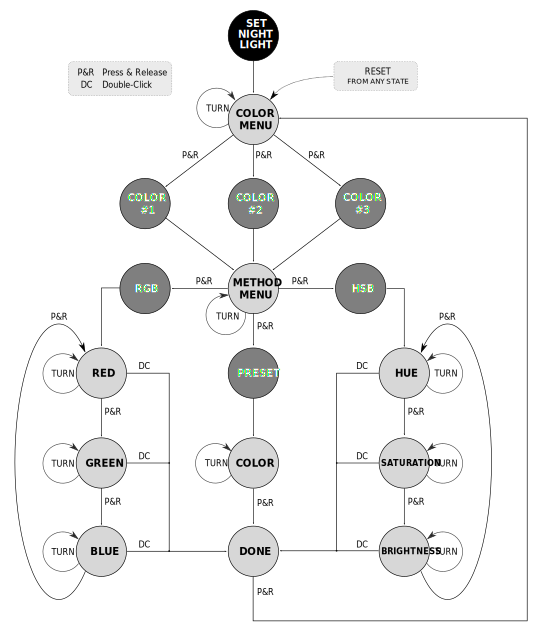
\includegraphics{images/set_night_light_state_diagram.png}
\caption{Set Night Light - State Diagram}
\end{figure}
